\subsection{Round 2 Solutions}\label{S::2022-O-2}

\begin{question}\label{A::2022-O-2-1}
    For $\triangle ABC$ and its circumcircle $\o$, draw the tangents at $B$, $C$ to $\o$ meeting at $D$. let the line $AD$ meet the circle with centre $D$ and radius $DB$ at $E$ inside $\triangle ABC$. Let $F$ be the point on the extension of $EB$ and $G$ be the point on the segment $EC$ such that $\angle AFB = \angle AGE = \angle A$. Prove that the tangent at $A$ to the circumcircle of $\triangle AFG$ is parallel to $BC$.
\end{question}

\resqh{https://artofproblemsolving.com/community/c6h2876083p25555411}{AoPS thread}

\solctt{https://artofproblemsolving.com/community/c6h2876083p25555460}{gghx}

\begin{center}
    \begin{tikzpicture}[scale=0.3]
        \coordinate[label=left:$O$] (O) at (0, 0);
        \coordinate[label=above left:$A$] (A) at (-10.941, 12.589);
        \coordinate[label=left:$B$] (B) at (-7.594, -14.850);
        \coordinate[label=right:$C$] (C) at (12.705, -10.806);
        \coordinate[label=below:$D$] (D) at (4.156, -20.859);
        \coordinate (E) at (-1.273, -8.830);
        \coordinate[label=left:$F$] (F) at (-15.954, -22.813);
        \coordinate (G) at (11.137, -10.584);
        \coordinate[label=below:$I$] (I) at (4.357, -3.468);
        \coordinate[label=above right:$J$] (J) at (-13.725, -7.071);

        \node at (-1.8, -10) {$E$};
        \node at (9, -9.7) {$G$};

        \draw[dashed] (O) circle[radius=16.679];
        \draw[dashed] (D) circle[radius=13.196];

        \draw (A) -- (B) -- (C) -- (A);
        \draw (B) -- (D) -- (C);
        \draw[very thick] (A) -- (F) -- (G) -- (A);
        \draw[dotted] (A) -- (D);
        \draw (J) -- (G);
        \draw (I) -- (F);
        \draw (E) -- (C);

        \draw[dotted] (B) -- (O) -- (C);

        \draw pic [draw, angle radius=12mm, ""] {angle = B--A--C};
        \draw pic [draw, angle radius=12mm, ""] {angle = A--G--E};
        \draw pic [draw, angle radius=12mm, ""] {angle = B--F--A};

        \fill (A) circle[radius=5pt];
        \fill (B) circle[radius=5pt];
        \fill (C) circle[radius=5pt];
        \fill (D) circle[radius=5pt];
        \fill (E) circle[radius=5pt];
        \fill (F) circle[radius=5pt];
        \fill (G) circle[radius=5pt];
        \fill (I) circle[radius=5pt];
        \fill (J) circle[radius=5pt];
        \fill (O) circle[radius=5pt];
    \end{tikzpicture}
\end{center}

\begin{claim}{1}
    $E$ is the orthocentre of $\triangle AFG$.
\end{claim}
\begin{proof}
    Let $O$ be the circumcentre of $\triangle ABC$. Let $I = AG \cap FE$ and $J = AF \cap GE$.

    Since $\angle BOC = 2\angle A$ and $\angle OBD = \angle OCD = 90\deg$, we have $\angle BDC = 180\deg - 2\angle A$, whence reflex $\angle BDC = 180\deg + 2\angle A$. Hence, $\angle BEC = 90\deg + \angle A$. This immediately gives \[\angle EIC + \angle AGE = 90\deg + \angle A \implies \angle EIC = 90\deg\] and \[\angle EJF + \angle AFB = 90\deg + \angle A \implies \angle EJF = 90\deg.\] Thus, $E$ is the orthocentre of $\triangle AFG$.
\end{proof}

\begin{center}
    \begin{tikzpicture}[scale=0.3]      
        \coordinate[label=above left:$A$] (A) at (-10.941, 12.589);
        \coordinate (B) at (-7.594, -14.850);
        \coordinate[label=right:$C$] (C) at (12.705, -10.806);
        \coordinate[label=below:$D$] (D) at (4.156, -20.859);
        \coordinate (E) at (-1.273, -8.830);
        \coordinate (G) at (11.137, -10.584);
        \coordinate[label=below left:$H$] (H) at (11.565, -11.033);
        \coordinate[label=right:$I$] (I) at (4.357, -3.468);

        \node at (-2.4, -8.5) {$E$};
        \node at (9, -9.7) {$G$};
        \node at (-8.7, -15.5) {$B$};

        \draw[dashed] (O) circle[radius=16.679];
        \draw[dashed] (D) circle[radius=13.196];

        \draw (B) -- (C);
        \draw (B) -- (D) -- (C);
        \draw (A) -- (H);
        \draw (A) -- (D);
        \draw (I) -- (B);
        \draw (E) -- (C);

        \draw pic [draw, angle radius=3mm, ""] {right angle = A--I--E};


        \fill (A) circle[radius=5pt];
        \fill (B) circle[radius=5pt];
        \fill (C) circle[radius=5pt];
        \fill (D) circle[radius=5pt];
        \fill (E) circle[radius=5pt];
        \fill (G) circle[radius=5pt];
        \fill (I) circle[radius=5pt];
        \fill (H) circle[radius=5pt];
    \end{tikzpicture}
\end{center}

Let $H = AG \cap BC$.
\begin{claim}{2}
    $AEHC$ is cyclic.
\end{claim}
\begin{proof}
    Note that $\triangle BDE$ is isosceles, with $\angle EBD = \angle BED$. Hence, $\angle BDE = 180\deg - 2\angle BED$. Thus, \[\angle GCH = \frac12 \angle BDE = 90\deg - \angle BED = 90\deg - \angle AEI = \angle GAE.\] Thus, by the converse of angles in same segment, $AEHC$ is cyclic.
\end{proof}

\clearpage
\begin{center}
    \begin{tikzpicture}[scale=0.3]
        \coordinate[label=above left:$A$] (A) at (-10.941, 12.589);
        \coordinate[label=right:$C$] (C) at (12.705, -10.806);
        \coordinate (E) at (-1.273, -8.830);
        \coordinate[label=below left:$F$] (F) at (-15.954, -22.813);
        \coordinate (G) at (11.137, -10.584);
        \coordinate[label=below:$H$] (H) at (11.565, -11.033);
        \coordinate[label=right:$T$] (T) at (9.362, 16.634);
        \coordinate[label=above right:$J$] (J) at (-13.725, -7.071);
        \coordinate[label=below right:$K$] (K) at (1.485, -14.941);

        \node at (-1.8, -10) {$E$};
        \node at (9, -9.7) {$G$};

        \draw[dashed] (-7.242, -5.991) circle[radius=18.944];

        \draw (G) -- (C) -- (A);
        \draw (A) -- (T);
        \draw (A) -- (H);
        \draw (A) -- (F) -- (G);
        \draw (A) -- (D);
        \draw (J) -- (C);
        \draw (H) -- (C);

        \fill (A) circle[radius=5pt];
        \fill (C) circle[radius=5pt];
        \fill (E) circle[radius=5pt];
        \fill (F) circle[radius=5pt];
        \fill (G) circle[radius=5pt];
        \fill (H) circle[radius=5pt];
        \fill (J) circle[radius=5pt];
        \fill (K) circle[radius=5pt];
        \fill (T) circle[radius=5pt];


        \draw pic [draw, angle radius=3mm, ""] {right angle = C--J--F};
        \draw pic [draw, angle radius=3mm, ""] {right angle = A--K--F};

        \draw pic [draw, angle radius=10mm, ""] {angle = C--F--A};
        \draw pic [draw, angle radius=10mm, ""] {angle = G--A--T};
    \end{tikzpicture}
\end{center}

\begin{claim}{3}
    The tangent at $A$ to $(AFG)$ is parallel to $HC$ (i.e. $BC$).
\end{claim}
\begin{proof}
    Let $K = AE \cap GF$. Let $T$ be a point on the line parallel to $HC$ through $A$, such that $G$ and $T$ are on the same side of $AE$. It suffices to show that $AT$ is tangent to $(AFG)$ at $A$.

    Observe that \[\angle TAG = 180\deg - \angle GHC = 180\deg - \angle GEA = 180\deg - \angle KEJ = \angle GFA.\] Thus, by the converse of the alternate segment theorem, $AT$ is tangent to $(AFG)$ at $A$.
\end{proof}
    
\begin{question}\label{A::2022-O-2-2}
    Prove that if the length and breadth of a rectangle are both odd integers, then there does not exist a point $P$ inside the rectangle such that each of the distances from $P$ to the 4 corners of the rectangle is an integer.
\end{question}

\resqh{https://artofproblemsolving.com/community/c6h2876084p25555412}{AoPS thread}

\solctt{https://artofproblemsolving.com/community/c6h2876084p25568028}{sarjinius} Let $m$ and $n$ be positive odd integers. Let $A(0, 0)$, $B(m, 0)$, $C(m, n)$ and $D(0, n)$. Let the perpendicular distance from $P$ to $AB$, $BC$, $CD$ and $DA$ be $a$, $b$, $c$ and $d$ respectively, whence $P(d, a)$. Also, we have $b + d = m$ and $a + c = n$. Seeking a contradiction, suppose $PA$, $PB$, $PC$ and $PD$ are all integers.

By Pythagoras' theorem, we have $PA^2 = a^2 + d^2$ and $PB^2 = a^2 + (m-d)^2$. Thus, both $a^2 + d^2$ and $a^2 + d^2 - 2md + m^2$ are perfect squares. This immediately gives \[d = \frac{m^2 + PA^2 - PB^2}{2m},\] whence $d$ is rational with a denominator not divisible by 4 (when expressed in lowest terms). Similarly, we also get \[a = \frac{n^2 + PB^2 - PC^2}{2n}, \quad b = \frac{m^2 + PC^2 - PD^2}{2m}, \quad c = \frac{n^2 + PD^2 - PA^2}{2n},\] thus $a$, $b$ and $c$ are also rational with denominator not divisible by 4.

By the British Flag theorem, we have $PA^2 + PC^2 = PB^2 + PD^2$. Thus, $PA^2 - PB^2 = -\bp{PC^2 - PD^2}$ and $PB^2 - PC^2 = -\bp{PD^2 - PA^2}$. It follows that $a$ and $c$ share the same denominator. Likewise, $b$ and $d$ share the same denominator. Let $k$ be the denominator of $a$ and $c$, and $l$ be the denominator of $b$ and $d$. Note that $k \mid 2n$ and $l \mid 2m$.

We now scale $ABCD$ with respect to $A$ by a factor of $\lcm{k, l}$ (note that this is not divisible by 4). Let $X_\ast$ represent the point $X$ after scaling and $z_\ast$ represent the distance $z$ after scaling.

\case{1} Suppose $\lcm{k, l}$ is odd. Thus, both $m_\ast$ and $n_\ast$ are odd. Since $a_\ast, b_\ast, c_\ast, d_\ast \in \ZZ$, with $b_\ast + d_\ast = m_\ast$ and $a_\ast + c_\ast = n_\ast$, it follows that one of $a$ and $c$ is odd, and one of $b$ and $d$ is odd. Hence, one of $PA_\ast^2 = a_\ast^2 + d_\ast^2$, $PB_\ast^2 = a_\ast^2 + b_\ast^2$, $PC_\ast^2 = c_\ast^2 + b_\ast^2$ and $PD_\ast^2 = c_\ast^2 + d_\ast^2$ must be 2 mod 4, which cannot be perfect square, a contradiction.

\case{1} Suppose $\lcm{k, l}$ is even. Then at least one of $k$ and $l$ is even (and also 2 mod 4). 

\subcase{2A} Suppose both $k$ and $l$ are even. This implies that $a_\ast$, $b_\ast$, $c_\ast$ and $d_\ast$ are all odd. This is a clear contradiction since the sum of two odd squares will always be 2 mod 4, which cannot be a perfect square.

\subcase{2B} Without loss of generality, suppose $k$ is odd and $l$ is even. Hence, $a_\ast$ and $c_\ast$ are even, while $b_\ast$ and $d_\ast$ are odd. However, because $a_\ast + c_\ast = n_\ast \equiv 2 \pmod{4}$, without loss of generality, we must have $a_\ast \equiv 0 \pmod{4}$ and $c_\ast \equiv 2 \pmod{4}$. Thus, $a_\ast^2 \equiv 0 \pmod{8}$ while $c_\ast^2 \equiv 4 \pmod{8}$. We also have $b_\ast^2 \equiv d_\ast^2 \equiv 1 \pmod{8}$. Thus, $PC_\ast^2 = c_\ast^2 + b_\ast^2$ and $PD_\ast^2 = c_\ast^2 + d_\ast^2$ must be 5 mod 8, which cannot be a perfect square, a contradiction. \qed

\begin{question}[${f(m) \equiv m}$]\label{A::2022-O-2-3}
    Find all functions $f : \ZZ^+ \to \ZZ^+$ satisfying \[m!! + n!! \mid f(m)!! + f(n)!!\] for each $m, n \in \ZZ^+$, where $n!! = (n!)!$ for all $n \in \ZZ^+$.
\end{question}

\resqh{https://artofproblemsolving.com/community/c6h2876085p25555413}{AoPS thread}

\solctt{https://artofproblemsolving.com/community/c6h2876085p25698517}{DVDthe1st} When $m = n$, we see that $m!! \mid f(m)!!$. This immediately gives us $f(m) \geq m$. Repeatedly chaining the given relation gives \[m!! + n!! \mid f(m)!! + f(n)!! \mid f^2(m)!! + f^2(n!!) \mid \cdots \mid f^k(m)!! + f^{k+1}(n)!!, \tag{1}\] where $k$ is a non-negative integer. We now consider the sequence $\bc{m, f(m), f^2(m), \ldots}$.

\case{1} Suppose the sequence is unbounded. Let $k > 0$ be the smallest integer such that $m!! + f(m)!! \mid f^{k+1}(m)!!$ ($k$ must exist due to the unboundedness of the sequence). To not violate the minimality of $k$, we must have $m!! + f(m)!! \nmid f^k(m)!!$. Thus, $m!! + f(m)!! \nmid f^k(m)!! + f^{k+1}(m)!!$, contradicting (1).

\case{2} Suppose the sequence is bounded. Let $k \geq 0$ be the smallest integer such that $f^k(m) = \max{m, f(m), f^2(m), \ldots}$. If $k > 0$, we have \[f^k(m)!! + f^{k+1}(m)!! \leq 2f^k(m)!! < 2\bp{f^{k-1}(m)!! + f^k(m)!!}.\] However, from (1), we see that \[f^{k-1}(m)!! + f^k(m)!! \mid f^k(m)!! + f^{k+1}(m).\] This immediately gives $f^{k-1}(m)!! + f^k(m)!! = f^k(m)!! + f^{k+1}(m)$, whence \[f^{k-1}(m) = f^{k+1}(m) \geq f^k(m),\] which violates the minimality of $k$. Thus, $k =0$, whence $f(m) \equiv m$ for any initial choice of $m \in \ZZ^+$, which clearly satisfies the given relation.
    
\begin{question}[$n-\gcd{n, k}$]\label{A::2022-O-2-4}
    Let $n$, $k$, $1 \leq k \leq n$ be fixed integers. Alice has $n$ cards in a row, where the card in position $i$ has the label $i + k$ (or $i + k - n$ if $i + k > n$). Alice starts by colouring each card either red or blue. Afterwards, she is allowed to make several moves, where each move consists of choosing two cards of different colours and swapping them. Find the minimum number of moves she has to make (given that she chooses the colouring optimally) to put the cards in order (i.e. card $i$ is at position $i$).
\end{question}

\resqh{https://artofproblemsolving.com/community/c6h2876086p25555417}{AoPS thread}

\solctt{https://artofproblemsolving.com/community/c6h2876086p25568807}{gghx} We claim that Alice requires a minimum of $n - \gcd{n, k}$ moves.

Consider a graph over vertices labelled 1 through $n$. If the card at position $i$ has label $j$, draw a directed edge from $i$ to $j$. Since each vertex has indegree 1 and outdegree 1, the graph is composed of disjoint cycles. We now consider the effect of swapping two cards (say, at positions $i$ and $j$) on our graph.

\begin{claim}{1}
    If the cards at $i$ and $j$ were initially in the same cycle, then the cycle will split into two cycles upon swapping the two cards.
\end{claim}
\begin{proof}
    Without loss of generality, let the cycle that $i$ and $j$ are in be \[(i', i, i'', \underbrace{\ldots}_{I}, j', j, j'', \underbrace{\ldots}_{J}).\] Consider the effect of swapping $i$ and $j$ on the cycle. Since the label on the card at position $i'$ is still $i$, we see that $i'$ still maps to $i$. Similarly, $j' \to j$. However, the card at position $j$ (originally at position $i$) now has the label $i''$, hence we now have $j \to i''$. Similarly, $i \to j''$. It is hence easy to see that the cycle now splits as \[(i', i, j'', \underbrace{\ldots}_{J})(j', j, i'', \underbrace{\ldots}_{I}).\]
\end{proof}

\begin{claim}{2}
    If the cards at $i$ and $j$ were initially in different cycles, then the two cycles will merge upon swapping the two cards.
\end{claim}
\begin{proof}
    Using a similar argument as Claim 1, the cycles \[(i', i, i'',. \underbrace{\ldots}_{I})\] and \[(j', j, j'', \underbrace{\ldots}_{J})\] will merge into a single cycle \[(i', i, j'', \underbrace{\ldots}_{J}, j', j, i'', \underbrace{\ldots}_{I})\] upon swapping positions $i$ and $j$.
\end{proof}

From Claims 1 and 2, it follows that every move, the number of cycles increases by at most one. We now show that the initial number of cycles is $\gcd{n, k}$.

\begin{claim}{3}
    The number of cycles is initially $\gcd{n, k}$.
\end{claim}
\begin{proof}
    Let $D = \bc{d \in \ZZ_n \mid 1 \leq d \leq \gcd{n, k}}$. Let $C(m)$ be the cycle starting from some integer $m$. Then $C(m)$ is clearly of the form \[(m, m+k, m+2k, m+3k, \ldots, m+(l-1)k),\] where $l = \frac{n}{\gcd{n, k}}$ is the smallest positive integer such that $lk \equiv 0 \pmod{n}$.

    Consider $C(m)$ for any choice of $m$. Since $k \equiv 0 \pmod{\gcd{n, k}}$, it follows that each member of $C(m)$ is congruent to $m$ $\pmod{\gcd{n, k}}$. In addition, from the minimality of $l$, all elements of $C(m)$ are distinct. Thus, there is exactly one $d \in D$ that is also in $C(m)$ (namely, $d \equiv m \pmod{\gcd{n, k}}$). Conversely, each $d \in D$ has a unique cycle $m$ that it is a member of. Hence, the number of cycles is $\gcd{n, k}$ as desired.
\end{proof}

Since there are $n$ cycles when all cards are in their correct position, Alice must make at least $n - \gcd{n, k}$ moves. We now construct a strategy that guarantees Alice can indeed win in $n -\gcd{n, k}$ moves.

\begin{claim}{4}
    Alice can win in $n - \gcd{n, k}$ moves.
\end{claim}
\begin{proof}
    Let all cards with labels $1, 2, \ldots, \gcd{n, k}$ be red, and all other cards be blue. By Claim 3, each cycle initially contains exactly one red card. For each cycle, keep swapping the red card with the card that is pointing towards it. Doing so removes one blue card every move. Since the cycle has length $\frac{n}{\gcd{n, k}}$, each cycle requires $\frac{n}{\gcd{n, k}} - 1$ moves to completely sort it. Since there are $\gcd{n, k}$ cycles to sort, Alice can sort all cycles within $n - \gcd{n, k}$ moves, as desired.
\end{proof}

As an example, consider the case where $n = 6$ and $k = 4$. We start with the following deck, which has been coloured using the strategy in Claim 4:

\begin{center}
    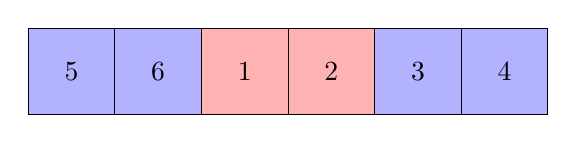
\begin{tikzpicture}
        \def \s {1.1}

        \draw[fill=blue!30] (0*\s, 0) rectangle ++ (\s, \s);
        \draw[fill=blue!30] (1*\s, 0) rectangle ++ (\s, \s);
        \draw[fill=red!30] (2*\s, 0) rectangle ++ (\s, \s);
        \draw[fill=red!30] (3*\s, 0) rectangle ++ (\s, \s);
        \draw[fill=blue!30] (4*\s, 0) rectangle ++ (\s, \s);
        \draw[fill=blue!30] (5*\s, 0) rectangle ++ (\s, \s);

        \node at (0.5*\s,0.5*\s) {5};
        \node at (1.5*\s,0.5*\s) {6};
        \node at (2.5*\s,0.5*\s) {1};
        \node at (3.5*\s,0.5*\s) {2};
        \node at (4.5*\s,0.5*\s) {3};
        \node at (5.5*\s,0.5*\s) {4};
    \end{tikzpicture}
\end{center}

The current cycles are $(1,5,3)(2,6,4)$. We first focus on the $(1,5,3)$ cycle. Since card 3 is pointing to card 1, we swap them:

\begin{center}
    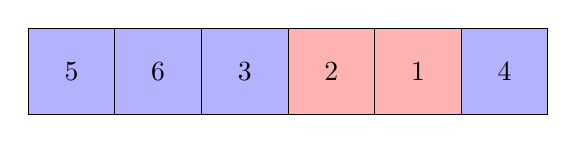
\begin{tikzpicture}
        \def \s {1.1}

        \draw[fill=blue!30] (0*\s, 0) rectangle ++ (\s, \s);
        \draw[fill=blue!30] (1*\s, 0) rectangle ++ (\s, \s);
        \draw[fill=blue!30] (2*\s, 0) rectangle ++ (\s, \s);
        \draw[fill=red!30] (3*\s, 0) rectangle ++ (\s, \s);
        \draw[fill=red!30] (4*\s, 0) rectangle ++ (\s, \s);
        \draw[fill=blue!30] (5*\s, 0) rectangle ++ (\s, \s);

        \node at (0.5*\s,0.5*\s) {5};
        \node at (1.5*\s,0.5*\s) {6};
        \node at (2.5*\s,0.5*\s) {3};
        \node at (3.5*\s,0.5*\s) {2};
        \node at (4.5*\s,0.5*\s) {1};
        \node at (5.5*\s,0.5*\s) {4};
    \end{tikzpicture}
\end{center}

The cycles are now $(1,5)(2,6,4)(3)$. Since card 5 is pointing to card 1, we swap them:

\begin{center}
    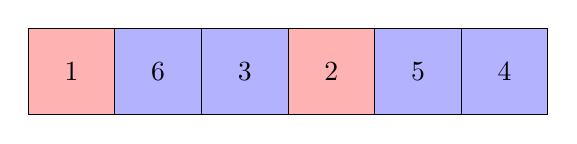
\begin{tikzpicture}
        \def \s {1.1}

        \draw[fill=red!30] (0*\s, 0) rectangle ++ (\s, \s);
        \draw[fill=blue!30] (1*\s, 0) rectangle ++ (\s, \s);
        \draw[fill=blue!30] (2*\s, 0) rectangle ++ (\s, \s);
        \draw[fill=red!30] (3*\s, 0) rectangle ++ (\s, \s);
        \draw[fill=blue!30] (4*\s, 0) rectangle ++ (\s, \s);
        \draw[fill=blue!30] (5*\s, 0) rectangle ++ (\s, \s);

        \node at (0.5*\s,0.5*\s) {1};
        \node at (1.5*\s,0.5*\s) {6};
        \node at (2.5*\s,0.5*\s) {3};
        \node at (3.5*\s,0.5*\s) {2};
        \node at (4.5*\s,0.5*\s) {5};
        \node at (5.5*\s,0.5*\s) {4};
    \end{tikzpicture}
\end{center}

At this point, the $(1,5,3)$ cycle has been completely sorted, taking $\frac{6}{{\gcd}{(6,4)}} - 1 = 2$ moves as expected. We now focus on the $(2,6,4)$ cycle. Since card 4 is pointing at card 2, we swap them:

\begin{center}
    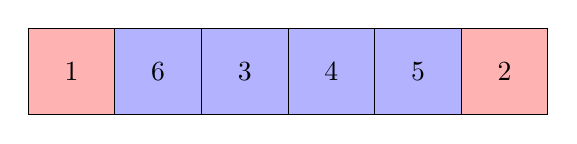
\begin{tikzpicture}
        \def \s {1.1}

        \draw[fill=red!30] (0*\s, 0) rectangle ++ (\s, \s);
        \draw[fill=blue!30] (1*\s, 0) rectangle ++ (\s, \s);
        \draw[fill=blue!30] (2*\s, 0) rectangle ++ (\s, \s);
        \draw[fill=blue!30] (3*\s, 0) rectangle ++ (\s, \s);
        \draw[fill=blue!30] (4*\s, 0) rectangle ++ (\s, \s);
        \draw[fill=red!30] (5*\s, 0) rectangle ++ (\s, \s);

        \node at (0.5*\s,0.5*\s) {1};
        \node at (1.5*\s,0.5*\s) {6};
        \node at (2.5*\s,0.5*\s) {3};
        \node at (3.5*\s,0.5*\s) {4};
        \node at (4.5*\s,0.5*\s) {5};
        \node at (5.5*\s,0.5*\s) {2};
    \end{tikzpicture}
\end{center}

Finally, we swap cards 2 and 6, completing the game in $6 - {\gcd}{(6,4)} = 4$ moves as expected.

\begin{center}
    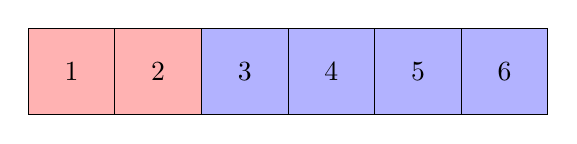
\begin{tikzpicture}
        \def \s {1.1}

        \draw[fill=red!30] (0*\s, 0) rectangle ++ (\s, \s);
        \draw[fill=red!30] (1*\s, 0) rectangle ++ (\s, \s);
        \draw[fill=blue!30] (2*\s, 0) rectangle ++ (\s, \s);
        \draw[fill=blue!30] (3*\s, 0) rectangle ++ (\s, \s);
        \draw[fill=blue!30] (4*\s, 0) rectangle ++ (\s, \s);
        \draw[fill=blue!30] (5*\s, 0) rectangle ++ (\s, \s);

        \node at (0.5*\s,0.5*\s) {1};
        \node at (1.5*\s,0.5*\s) {2};
        \node at (2.5*\s,0.5*\s) {3};
        \node at (3.5*\s,0.5*\s) {4};
        \node at (4.5*\s,0.5*\s) {5};
        \node at (5.5*\s,0.5*\s) {6};
    \end{tikzpicture}
\end{center}

\begin{question}\label{A::2022-O-2-5}
    Let $n \geq 2$ be a positive integer. For any integer $a$, let $P_a(x)$ denote the polynomial $x^n + ax$. Let $p$ be a prime number and define the set $S_a$ as the set of residues mod $p$ that $P_a(x)$ attains. That is, \[S_a = \bc{b \mid 0 \leq b \leq p -1, \text{ and there is $c$ such that $P_a(x) \equiv p \pmod{p}$}}.\] Show that the expression $\frac1{p-1} \sum_{a=1}^{p-1} \abs{S_a}$ is an integer.
\end{question}

\resqh{https://artofproblemsolving.com/community/c6h2876088p25555422}{AoPS thread}

\solcit{https://artofproblemsolving.com/community/c6h2876088p28594891}{Evan Chen} Note that $0 \in S_a$ for all integers $a \in [1, p-1]$. We thus consider only non-zero elements of $S_a$. Observe that \[\abs{S_1 \setminus \bc{0}} + \abs{S_2 \setminus \bc{0}} + \abs{S_3 \setminus \bc{0}} + \cdots + \abs{S_{p-1} \setminus \bc{0}}\] counts the number of elements in \[\mathcal{T} = \bc{(y, a) \in \FF_p^\times \times \FF_p^\times \mid \exists x \in \FF_p, y = x^n + ax}.\] Because $y = x^n + ax$ implies that $\l^n y = (\l x)^n + (\l^{n-1} a)(\l x)$ for any $\l \in \FF_p^\times$, we have the equivalence relation \[(y, a) \sim (\l^n y, \l^{n-1} a).\] Now observe that the pairs $(\l^n y, \l^{n-1} a)$ are pairwise distinct: \[(\l_1^n y, \l_1^{n-1} a) = (\l_2^n y, \l_2^{n-1} a) \implies \l_1^n \equiv \l_2^n \text{ and } \l_1^{n-1} \equiv \l_2^{n-1} \implies \l_1 = \l_2.\] Since there are $p-1$ choices of $\l$, each equivalence class generated by the above equivalence relation has exactly $p-1$ elements, whence $\abs{\mathcal{T}}$ is divisible by $p-1$. \qed

\begin{remark}
    The condition $n \geq 2$ ensures that we can split $\l^n$ into $\l^{n-1} \cdot \l$ to form the equivalence relation.
\end{remark}

\begin{remark}
    This question is identical to \hyperref[A::2023-O-2-3]{2023 Open Round 2 Question 3}.
\end{remark}
